%%%%%%%%%%%%%%%%%%%%%%%%%%%%%%%%%%%%%%%%%
% Beamer Presentation
% LaTeX Template
% Version 1.0 (10/11/12)
%
% This template has been downloaded from:
% http://www.LaTeXTemplates.com
%
% License:
% CC BY-NC-SA 3.0 (http://creativecommons.org/licenses/by-nc-sa/3.0/)
%
%%%%%%%%%%%%%%%%%%%%%%%%%%%%%%%%%%%%%%%%%

%-------------------------------------------------------------------------------
%	PACKAGES AND THEMES
%-------------------------------------------------------------------------------

\documentclass{beamer}
\usepackage{xcolor}
\usepackage{graphicx}
\usepackage{tikz}
\usepackage{listings}
\usepackage{multicol}

\DeclareMathOperator{\diag}{diag}

\definecolor{applegreen}{rgb}{0.55, 0.71, 0.0}
\definecolor{blue(ncs)}{rgb}{0.0, 0.45, 0.60}
\definecolor{burgundy}{rgb}{0.5, 0.0, 0.13}

\definecolor{cadet}{rgb}{0.33, 0.41, 0.47}
\definecolor{airforceblue}{rgb}{0.36, 0.54, 0.66}

\mode<presentation> {

\usetheme{CambridgeUS}

\usecolortheme{wolverine}

\definecolor{gold}{HTML}{D4A017}
\definecolor{darkgold}{HTML}{B7950B}

\setbeamercolor{palette primary}{bg=cadet,fg=white}
\setbeamercolor{palette secondary}{bg=airforceblue,fg=white}
\setbeamercolor{palette tertiary}{bg=black,fg=white}
\setbeamercolor{palette quaternary}{bg=cadet,fg=white}

\setbeamercolor{frametitle}{bg=airforceblue,fg=white}

\setbeamercolor{section number projected}{bg=black,fg=cadet}
\setbeamercolor{item}{fg=black,bg=cadet}

\setbeamertemplate{page number in head/foot}[framenumber]

\lstset{basicstyle=\ttfamily\footnotesize,breaklines=true}
}



\lstdefinestyle{colouredC}{ 
  commentstyle=\color[gray]{0.4},
  keywordstyle=\bfseries,
  keywordstyle=[2]\color[rgb]{0.75, 0, 0},
  keywordstyle=[3]\color[rgb]{0, 0.5, 0},
  keywordstyle=[4]\color[rgb]{0, 0.5, 0},
  keywordstyle=[5]\color[rgb]{0, 0, 0.75},
  numberstyle=\tiny\color{mGray},
  stringstyle=\color[rgb]{0, 0, 0.5},
  basicstyle=\ttfamily,
  language=C,
  morekeywords=[3]{CeedInt, CeedScalar},
}

\lstdefinestyle{boxedC}{
  style=colouredC,
  numbers=left,
  firstnumber=auto,
  numberblanklines=true,
  frame=trbL,
  numberstyle=\tiny,
  frame=leftline,
  numbersep=7pt,
  framesep=5pt,
  framerule=10pt,
  xleftmargin=15pt,
  backgroundcolor=\color[gray]{0.97},
  rulecolor=\color[gray]{0.90}%
}

\usepackage{graphicx} % Allows including images
\usepackage{booktabs} % Allows the use of \toprule, \midrule and \bottomrule in tables

%----------------------------------------------------------------------------------------
%	TITLE PAGE
%----------------------------------------------------------------------------------------

\title[libCEED]{libCEED GPU Strategy
} % The short title appears at the bottom of every slide, the full title is only on the title page

\author{Jeremy L Thompson} % Your name
\institute[CU Boulder] % Your institution as it will appear on the bottom of every slide, may be shorthand to save space
{University of Colorado Boulder \\ % Your institution for the title page
\medskip
\textit{jeremy@jeremylt.org} % Your email addressintention
}
\date{11 Feb 2025} % Date, can be changed to a custom date

\begin{document}

\begin{frame}
\titlepage % Print the title page as the first slide
\end{frame}

%------------------------------------------------

\begin{frame}
\frametitle{libCEED, Ratel, and HONEE Team}

\begin{center}
\includegraphics[height=2.75cm]{libCEEDlogo.png}
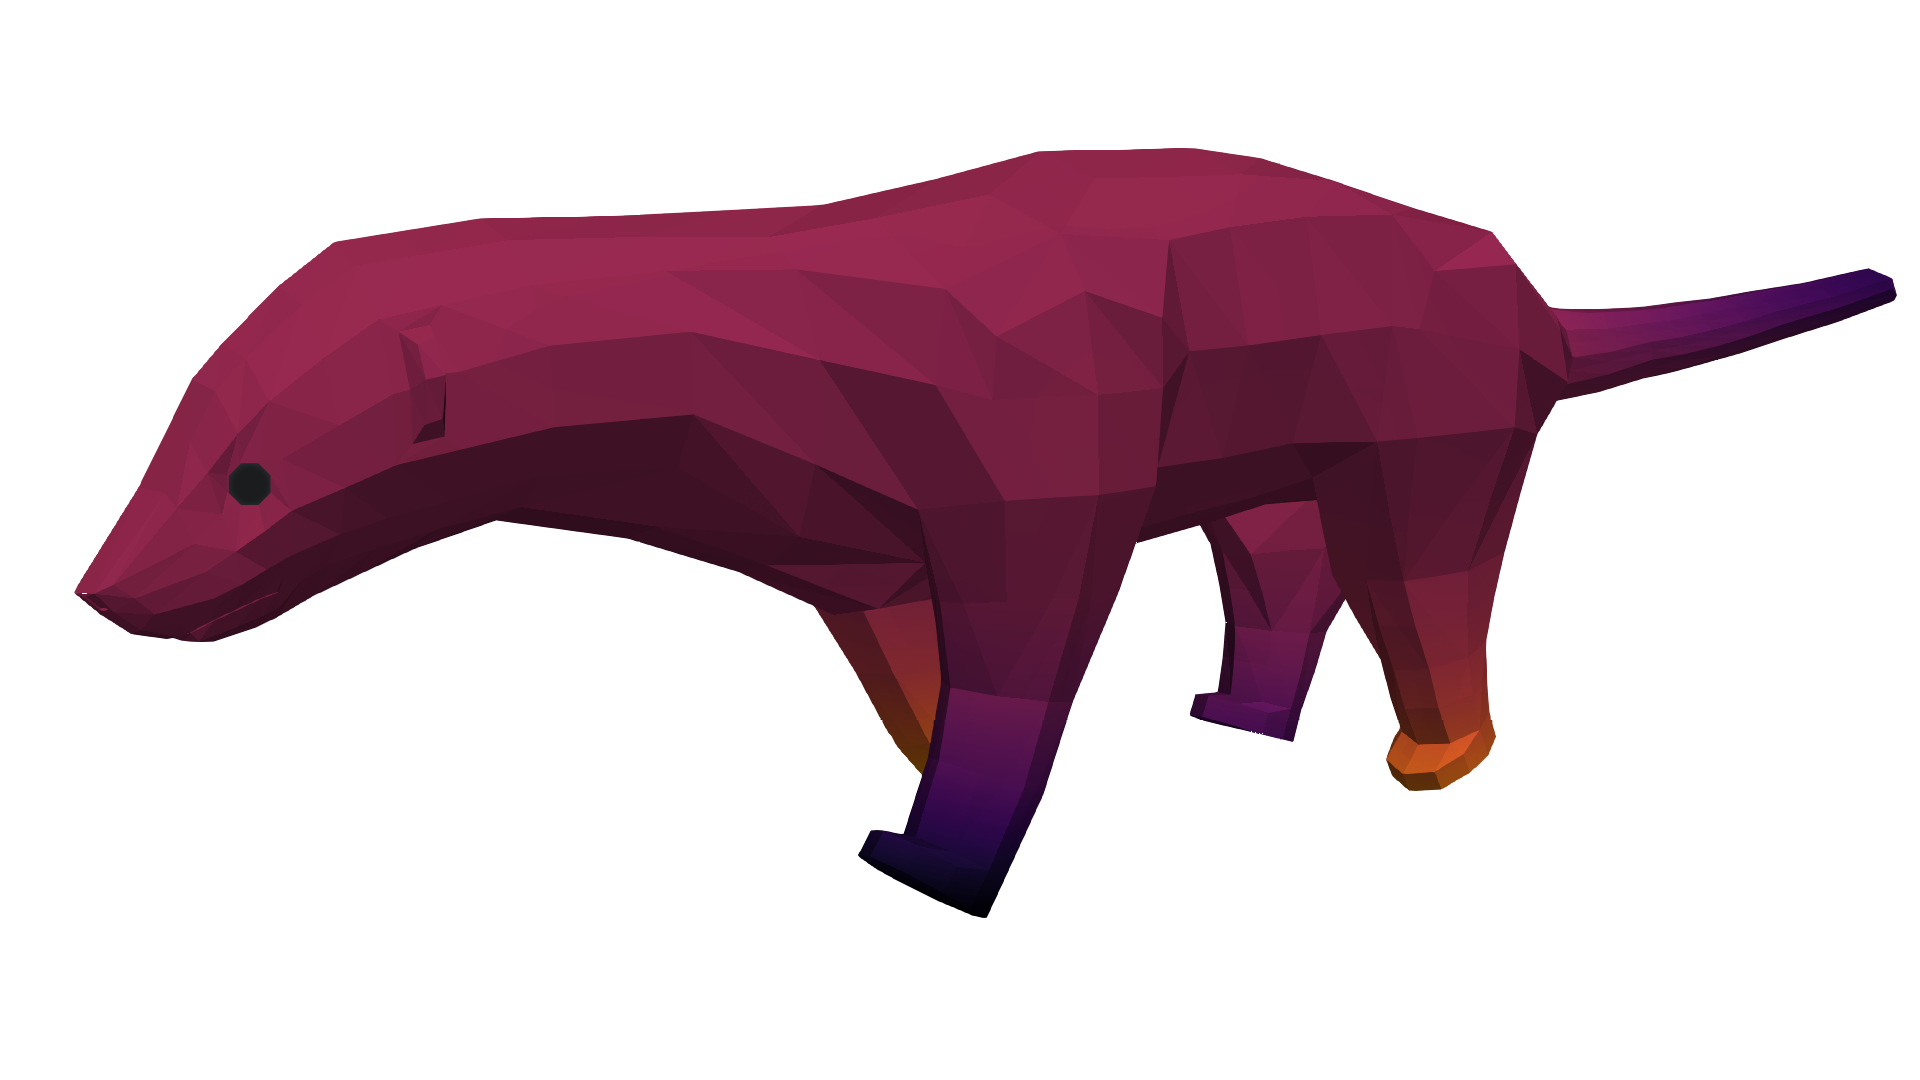
\includegraphics[height=2.75cm]{Ratellogo.png}
\end{center}

{\flushleft

libCEED Repo: https://github.com/CEED/libCEED\\
HONEE Repo: https://gitlab.com/phypid/HONEE\\
Ratel Repo: https://gitlab.com/micromorph/ratel\\

~\\
Developers: \textbf{Zach Atkins}, Jed Brown, Fabio Di Gioacchino, Leila Ghaffari,\\
\hspace{19mm} Kenneth Jansen, \textbf{Rezgar Shakeri}, James Wright,\\
\hspace{19mm} \textbf{Jeremy L Thompson}\\

~\\

{\tiny The authors acknowledge support by the Department of Energy, National Nuclear Security Administration, Predictive Science\\Academic Alliance Program (PSAAP) under Award Number DE-NA0003962.}

}

\begin{center}

\includegraphics[height=0.7cm]{psaap-center-logos}
\end{center}

\end{frame}

%------------------------------------------------

\begin{frame}
\frametitle{Overview} % Table of contents slide, comment this block out to remove it
\tableofcontents % Throughout your presentation, if you choose to use \section{} and \subsection{} commands, these will automatically be printed on this slide as an overview of your presentation
\end{frame}

%------------------------------------------------
\section{Background}
%------------------------------------------------

\begin{frame}
\begin{center}
\frametitle{ECP Roots}

\begin{itemize}

\item libCEED + PETSc projects follow from ECP CEED work\\

~\\

\item libCEED provides high-performance operator evaluation\\

~\\

\item libCEED provides CUDA, ROCm, and SYCL support\\

~\\

\item PETSc provides linear/non-linear solvers and time steppers\\

\end{itemize}

\end{center}
\end{frame}

%-------------------------------------------------------------------------------

\begin{frame}
\begin{center}
\frametitle{libCEED Projects}

Several projects built using libCEED\\

~\\

\begin{itemize}

\item Ratel - solid mechanics FEM and MPM (PSAAP)\\

~\\

\item HONEE - fluid dynamics FEM \& differential filtering (PHASTA)\\

~\\

\item MFEM - various applications, libCEED integrators (LLNL)\\

~\\

\item Palace - Electromagnetics FEM with MFEM + libCEED (Amazon)\\

~\\

\item RDycore - River dynamical core with PETSc + libCEED (SciDAC)\\

\end{itemize}

\end{center}
\end{frame}

%------------------------------------------------

\begin{frame}
\begin{center}
\frametitle{Matrix-Free Operators from libCEED}

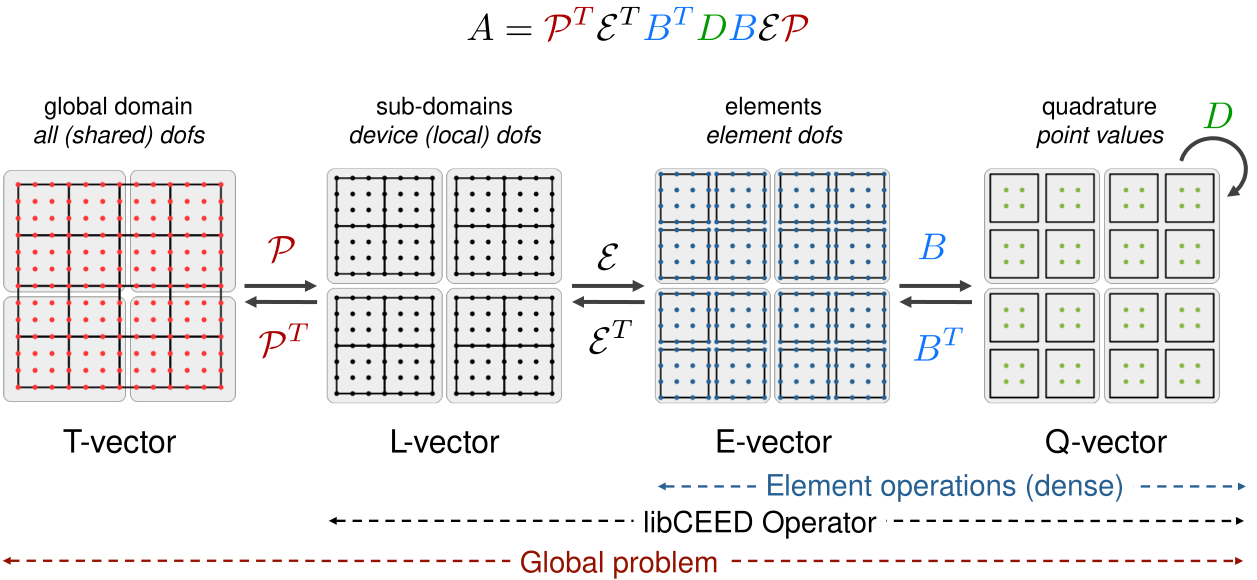
\includegraphics[height=5.0cm]{libCEEDAPI.png}

~\\

libCEED provides arbitrary order matrix-free operator evaluation\\

\end{center}
\end{frame}

%------------------------------------------------

\begin{frame}
\begin{center}
\frametitle{Performance Portability from libCEED}

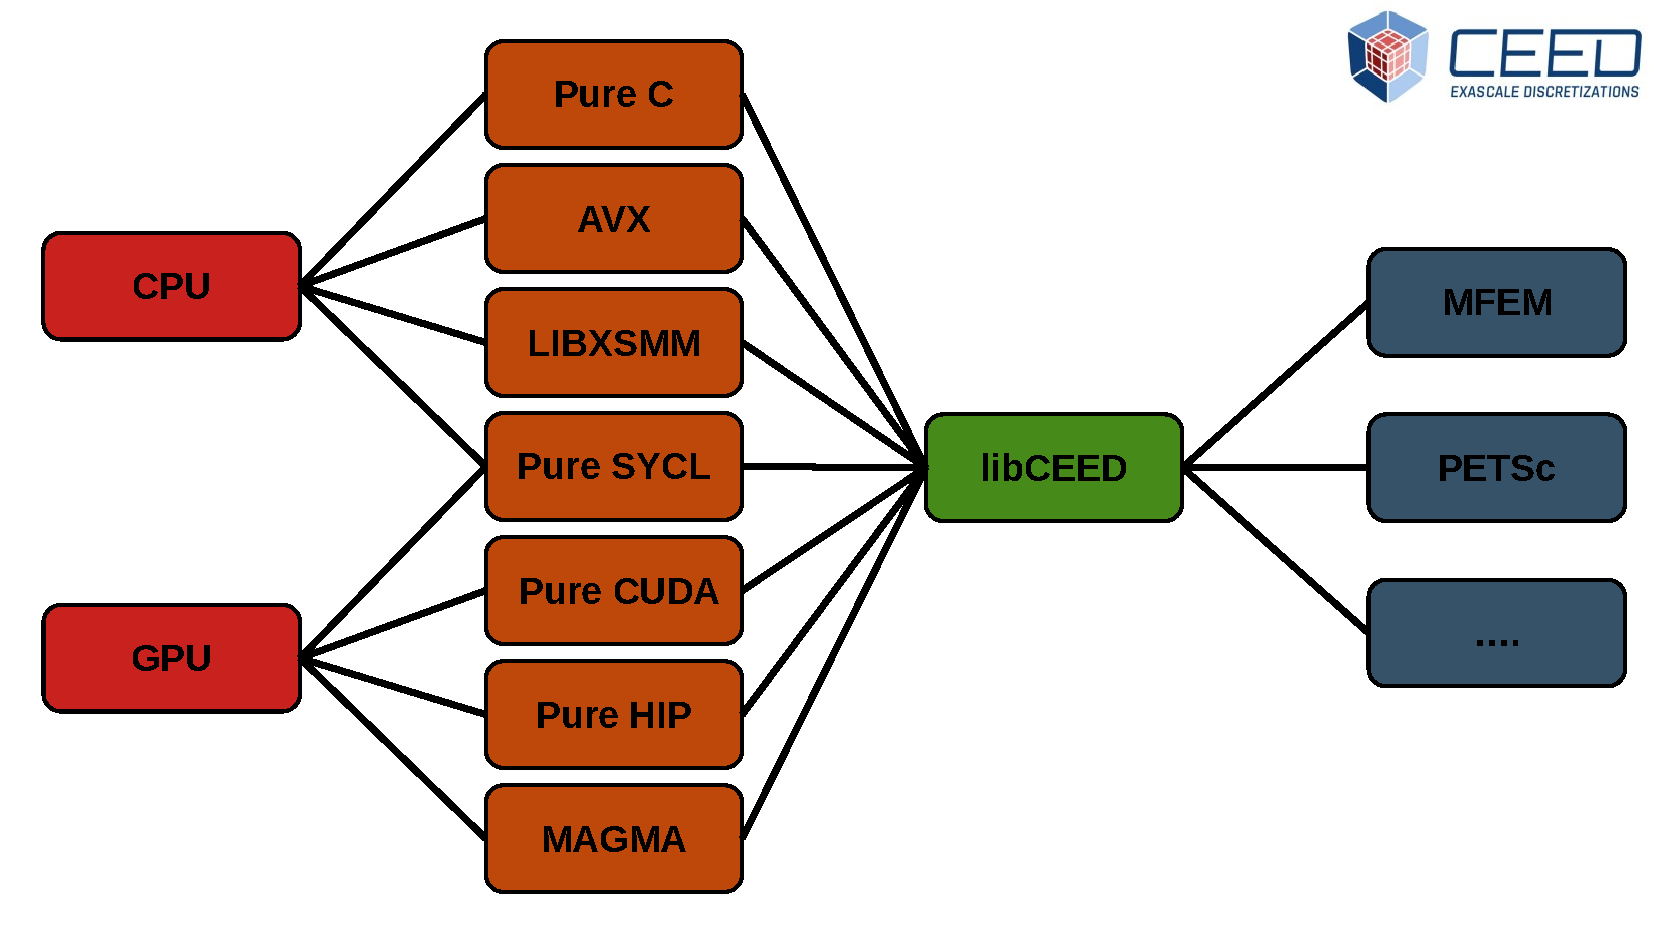
\includegraphics[height=5.5cm]{libCEEDBackends.pdf}

~\\

libCEED backends target different hardware at runtime\\

\end{center}
\end{frame}

%------------------------------------------------

\begin{frame}[fragile]
\begin{center}
\frametitle{Extensible Solvers from PETSc}

\begin{columns}
  \begin{column}{.25\textwidth}
    ~\\
    \lstinline{CeedEvaluator}\\
    \vspace{1.75cm}
    \lstinline{MatCeed}\\
    \vspace{0.75cm}
    \lstinline{CeedVector}\\
  \end{column}
  \begin{column}{.75\textwidth}
    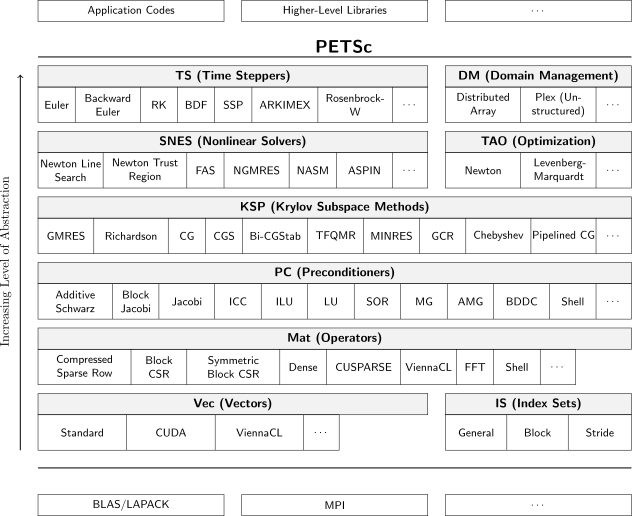
\includegraphics[height=6.0cm]{PETScAPI.png}
  \end{column}
\end{columns}

~\\

libCEED provides the local operator action for PETSc objects\\

\end{center}
\end{frame}

%------------------------------------------------
\section{General GPU Strategy}
%------------------------------------------------

\begin{frame}[fragile]
\begin{center}
\frametitle{Two Families of Approaches}

Three libCEED backends with two approaches to operator application\\

~\\

\begin{itemize}

\item Separate kernels

\begin{itemize}

\item \lstinline{/gpu/*/ref} and \lstinline{/gpu/*/shared}\\

~\\

\item $\mathcal{E}$, {\color{blue(ncs)}$B$}, and {\color{applegreen}$D$} all separate kernels\\

~\\

\item Higher overall memory usage, multiple kernel launches\\

~\\

\end{itemize}

\item Fused kernel

\begin{itemize}

\item \lstinline{/gpu/*/gen}\\

~\\

\item Single kernel JiTed with data from $\mathcal{E}$, {\color{blue(ncs)}$B$}, and {\color{applegreen}$D$}\\

~\\

\item Lower overall memory usage, single kernel launch\\

\end{itemize}

\end{itemize}

\end{center}
\end{frame}


%------------------------------------------------
\subsection{Ref Operators}
%------------------------------------------------

\begin{frame}[fragile]
\begin{center}
\frametitle{Ref Operator Application}

\lstinline{/gpu/*/ref} and \lstinline{/gpu/*/shared} use largely the same code\\

~\\

${\color{burgundy}A}_L = \mathcal{E}^T {\color{blue(ncs)}B}^T {\color{applegreen}D} {\color{blue(ncs)}B} \mathcal{E}$ use separate kernels\\

~\\

$\mathcal{E}$ source comes from the \lstinline{/gpu/*/ref}\\

~\\

\lstinline{/gpu/*/ref} uses basic kernels for {\color{blue(ncs)}$B$}\\

~\\

\lstinline{/gpu/*/shared} uses shared memory for {\color{blue(ncs)}$B$}\\

~\\

{\color{applegreen}$D$} source is given by the user\\

\end{center}
\end{frame}

%------------------------------------------------
\subsection{Shared Memory Bases}
%------------------------------------------------

\begin{frame}[fragile]
\begin{center}
\frametitle{Shared Basis Code}

{\tiny
\begin{lstlisting}[style=boxedC]
extern "C" __launch_bounds__(BASIS_GRAD_BLOCK_SIZE) __global__
    void Grad(const CeedInt num_elem, const CeedScalar *c_B,
    const CeedScalar *c_G, const CeedScalar *__restrict__ d_U,
    CeedScalar *__restrict__ d_V) {
  // Setup (omitted)
  // Apply basis element by element
  for (CeedInt elem=blockIdx.x*blockDim.z+threadIdx.z; elem<num_elem; elem+=gridDim.x*blockDim.z) {
    ReadElementStrided2d<NUM_COMP,P_1D>(data,elem,1,P_1D*P_1D*num_elem,P_1D*P_1D,d_U,r_U);
    GradTensor2d<NUM_COMP,P_1D,Q_1D>(data,r_U,s_B,s_G,r_V);
    WriteElementStrided2d<NUM_COMP*DIM,Q_1D>(data,elem,1,Q_1D*Q_1D*num_elem,Q_1D*Q_1D,r_V,d_V);
  }
}
\end{lstlisting}
}

$x$ and $y$ thread index gives point (2D) or column of points (3D)\\

~\\

$z$ thread index gives the element\\

\end{center}
\end{frame}

%------------------------------------------------

\begin{frame}
\begin{center}
\frametitle{Thread Usage}

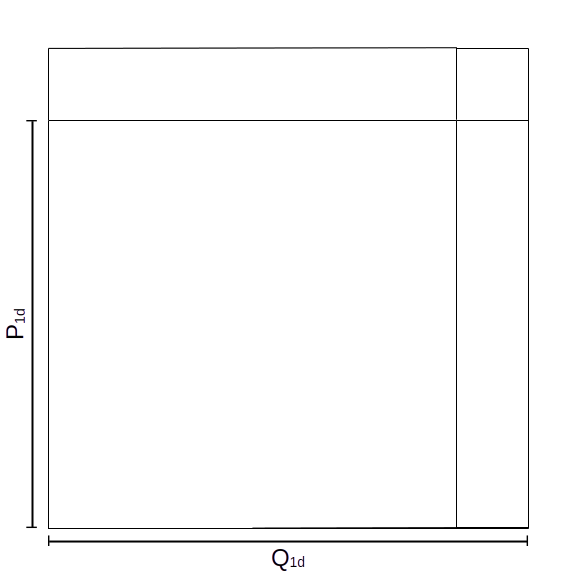
\includegraphics[height=5.0cm]{threadblockDiagram.png}

\includegraphics[height=5.0cm]{3DSlicing.png}

~\\

$x$ and $y$ thread index gives point (2D) or column of points (3D)\\

~\\

3D strategy works on 2D slabs of points\\

\end{center}
\end{frame}

%------------------------------------------------

\begin{frame}[fragile]
\begin{center}
\frametitle{Shared Basis Code}

{\tiny
\begin{lstlisting}[style=boxedC]
template <int NUM_COMP, int P_1D, int Q_1D>
inline __device__ void GradTensor2d(SharedData_Hip &data,
    const CeedScalar *__restrict__ r_U, const CeedScalar *c_B,
    const CeedScalar *c_G, CeedScalar *__restrict__ r_V) {
  CeedScalar r_t[1];
  for (CeedInt comp = 0; comp < NUM_COMP; comp++) {
    ContractX2d<NUM_COMP,P_1D,Q_1D>(data, &r_U[comp], c_G, r_t);
    ContractY2d<NUM_COMP,P_1D,Q_1D>(data, r_t, c_B, &r_V[comp+0*NUM_COMP]);
    ContractX2d<NUM_COMP,P_1D,Q_1D>(data, &r_U[comp], c_B, r_t);
    ContractY2d<NUM_COMP,P_1D,Q_1D>(data, r_t, c_G, &r_V[comp+1*NUM_COMP]);
  }
}

template <int NUM_COMP, int P_1D, int Q_1D>
inline __device__ void GradTransposeTensor2d(SharedData_Hip &data,
    const CeedScalar *__restrict__ r_U, const CeedScalar *c_B,
    const CeedScalar *c_G, CeedScalar *__restrict__ r_V) {
  CeedScalar r_t[1];
  for (CeedInt comp = 0; comp < NUM_COMP; comp++) {
    ContractTransposeY2d<NUM_COMP,P_1D,Q_1D>(data, &r_U[comp+0*NUM_COMP], c_B, r_t);
    ContractTransposeX2d<NUM_COMP,P_1D,Q_1D>(data, r_t, c_G, &r_V[comp]);
    ContractTransposeY2d<NUM_COMP,P_1D,Q_1D>(data, &r_U[comp+1*NUM_COMP], c_G, r_t);
    ContractTransposeAddX2d<NUM_COMP,P_1D,Q_1D>(data, r_t, c_B, &r_V[comp]);
  }
}

\end{lstlisting}
}

Loop over components to reduce total shared memory needed\\

\end{center}
\end{frame}

%------------------------------------------------

\begin{frame}[fragile]
\begin{center}
\frametitle{Shared Basis Code}

{\tiny
\begin{lstlisting}[style=boxedC]
template <int NUM_COMP, int P_1D, int Q_1D>
inline __device__ void ContractX3d(SharedData_Hip &data, const CeedScalar *U,
    const CeedScalar *B, CeedScalar *V) {
  CeedScalar r_B[P_1D];
  for (CeedInt i = 0; i < P_1D; i++) r_B[i] = B[i + data.t_id_x * P_1D];

  for (CeedInt k = 0; k < P_1D; k++) {
    data.slice[data.t_id_x + data.t_id_y * T_1D] = U[k];
    __syncthreads();
    V[k] = 0.0;
    if (data.t_id_x < Q_1D && data.t_id_y < P_1D) {
      for (CeedInt i = 0; i < P_1D; i++) {
        V[k] += r_B[i] * data.slice[i + data.t_id_y * T_1D];
      }
    }
    __syncthreads();
  }
}
\end{lstlisting}
}

Each thread computes all node's contributions to one quadrature point\\

~\\

3D loops over 2D slabs for tensor contraction\\

\end{center}
\end{frame}

%------------------------------------------------
\subsection{Gen Operators}
%------------------------------------------------

\begin{frame}[fragile]
\begin{center}
\frametitle{Gen Operator Application}

\lstinline{/gpu/*/gen} generates a single kernel for the operator\\

~\\

${\color{burgundy}A}_L = \mathcal{E}^T {\color{blue(ncs)}B}^T {\color{applegreen}D} {\color{blue(ncs)}B} \mathcal{E}$ uses a single kernel\\

~\\

$\mathcal{E}$ source comes from the \lstinline{/gpu/*/ref}\\

~\\

{\color{blue(ncs)}$B$} source comes from \lstinline{/gpu/*/shared}\\

~\\

{\color{applegreen}$D$} source is given by the user\\

\end{center}
\end{frame}

%------------------------------------------------

\begin{frame}[fragile]
\begin{center}
\frametitle{Generated Operator Kernel}

{\tiny
\begin{lstlisting}[style=boxedC]
extern "C" __global__ void CeedKernelCudaGenOperator_mass(CeedInt num_elem,
    void* ctx, FieldsInt_Cuda indices, Fields_Cuda fields, Fields_Cuda B,
    Fields_Cuda G, CeedScalar *W, Points_Cuda points) {
  // Setup kernel data

  // Input and Output field constants and basis data

  // Element loop
  __syncthreads();
  for (CeedInt elem = blockIdx.x*blockDim.z + threadIdx.z; elem < num_elem; elem += gridDim.x*blockDim.z) {
    // -- Input field restrictions (E) and basis actions (B)

    // -- Output field setup
    {
      // -- Apply QFunction (D)
      mass(ctx, 1, inputs, outputs);
    }

    // -- Output field basis actions (B^T) and restrictions (E^T)
  }
}
// -----------------------------------------------------------------------------

\end{lstlisting}
}

${\color{burgundy}A}_L = \mathcal{E}^T {\color{blue(ncs)}B}^T {\color{applegreen}D} {\color{blue(ncs)}B} \mathcal{E}$ in a single kernel\\

\end{center}
\end{frame}

%------------------------------------------------

\begin{frame}[fragile]
\begin{center}
\frametitle{Generated Operator Kernel}

{\tiny
\begin{lstlisting}[style=boxedC]
  // Setup kernel data
  const CeedScalar *d_in_0 = fields.inputs[0];
  const CeedScalar *d_in_1 = fields.inputs[1];
  CeedScalar *d_out_0 = fields.outputs[0];
  const CeedInt dim = 1;
  const CeedInt Q_1d = 8;
  extern __shared__ CeedScalar slice[];
  SharedData_Cuda data;
  data.t_id_x = threadIdx.x;
  data.t_id_y = threadIdx.y;
  data.t_id_z = threadIdx.z;
  data.t_id  = threadIdx.x+threadIdx.y*blockDim.x+threadIdx.z*blockDim.y*blockDim.x;
  data.slice = slice + data.t_id_z*T_1D;

\end{lstlisting}
}

Set up pointers to basis data and shared memory\\

\end{center}
\end{frame}

%------------------------------------------------

\begin{frame}[fragile]
\begin{center}
\frametitle{Generated Operator Kernel}

{\tiny
\begin{lstlisting}[style=boxedC]
  // Input field constants and basis data
  // -- Input field 0
  const CeedInt P_1d_in_0 = 8;
  const CeedInt num_comp_in_0 = 1;
  // EvalMode: none
  // -- Input field 1
  const CeedInt P_1d_in_1 = 5;
  const CeedInt num_comp_in_1 = 1;
  // EvalMode: interpolation
  __shared__ CeedScalar s_B_in_1[40];
  LoadMatrix<P_1d_in_1, Q_1d>(data, B.inputs[1], s_B_in_1);

  // Output field constants and basis data
  // -- Output field 0
  const CeedInt P_1d_out_0 = 5;
  const CeedInt num_comp_out_0 = 1;
  // EvalMode: interpolation
  __shared__ CeedScalar s_B_out_0[40];
  LoadMatrix<P_1d_out_0, Q_1d>(data, B.outputs[0], s_B_out_0);
\end{lstlisting}
}

Basis data and constants loaded\\

\end{center}
\end{frame}

%------------------------------------------------

\begin{frame}[fragile]
\begin{center}
\frametitle{Generated Operator Kernel}

{\tiny
\begin{lstlisting}[style=boxedC]
    // Scratch restriction buffer space
    CeedScalar r_e_scratch[8];

    // -- Input field restrictions and basis actions
    // ---- Input field 0
    CeedScalar r_e_in_0[num_comp_in_0*P_1d_in_0];
    // Strides: {1, 8, 8}
    ReadLVecStrided1d<num_comp_in_0, P_1d_in_0,1,8,8>(data, elem, d_in_0, r_e_in_0);
    // EvalMode: none
    CeedScalar *r_q_in_0 = r_e_in_0;
    // ---- Input field 1
    CeedScalar *r_e_in_1 = r_e_scratch;
    const CeedInt l_size_in_1 = 61;
    // CompStride: 1
    ReadLVecStandard1d<num_comp_in_1, 1, P_1d_in_1>(data, l_size_in_1, elem, indices.inputs[1], d_in_1, r_e_in_1);
    // EvalMode: interpolation
    CeedScalar r_q_in_1[num_comp_in_1*Q_1d];
    Interp1d<num_comp_in_1, P_1d_in_1, Q_1d>(data, r_e_in_1, s_B_in_1, r_q_in_1);

    // -- Output field setup
    // ---- Output field 0
    CeedScalar r_q_out_0[num_comp_out_0*Q_1d];

\end{lstlisting}
}

Restrict and apply basis for each input\\

~\\

Setup output data buffers\\

\end{center}
\end{frame}

%------------------------------------------------

\begin{frame}[fragile]
\begin{center}
\frametitle{Generated Operator Kernel}

{\tiny
\begin{lstlisting}[style=boxedC]
    // Note: Using full elements
    {
      // -- Input fields
      // ---- Input field 0
      CeedScalar *r_s_in_0 = r_q_in_0;
      // ---- Input field 1
      CeedScalar *r_s_in_1 = r_q_in_1;
      // -- Output fields
      // ---- Output field 0
      CeedScalar *r_s_out_0 = r_q_out_0;

      // -- QFunction inputs and outputs
      // ---- Inputs
      CeedScalar *inputs[2];
      // ------ Input field 0
      inputs[0] = r_s_in_0;
      // ------ Input field 1
      inputs[1] = r_s_in_1;
      // ---- Outputs
      CeedScalar *outputs[1];
      // ------ Output field 0
      outputs[0] = r_s_out_0;

      // -- Apply QFunction
      mass(ctx, 1, inputs, outputs);
    }

\end{lstlisting}
}

Apply QFunction at each quadrature point\\

May apply to 2D slabs or full elements in 3D\\

\end{center}
\end{frame}

%------------------------------------------------

\begin{frame}[fragile]
\begin{center}
\frametitle{Generated Operator Kernel}

{\tiny
\begin{lstlisting}[style=boxedC]
    // -- Output field basis action and restrictions
    // ---- Output field 0
    // EvalMode: interpolation
    CeedScalar *r_e_out_0 = r_e_scratch;
    InterpTranspose1d<num_comp_out_0, P_1d_out_0, Q_1d>(data, r_q_out_0, s_B_out_0, r_e_out_0);
    const CeedInt l_size_out_0 = 61;
    // CompStride: 1
    WriteLVecStandard1d<num_comp_out_0, 1, P_1d_out_0>(data, l_size_out_0, elem, indices.outputs[0], r_e_out_0, d_out_0);
\end{lstlisting}
}

Output basis action and restriction to assemble result\\

\end{center}
\end{frame}

%------------------------------------------------
\section{MPM Support}
%------------------------------------------------

\begin{frame}
\begin{center}
\frametitle{What is MPM?}

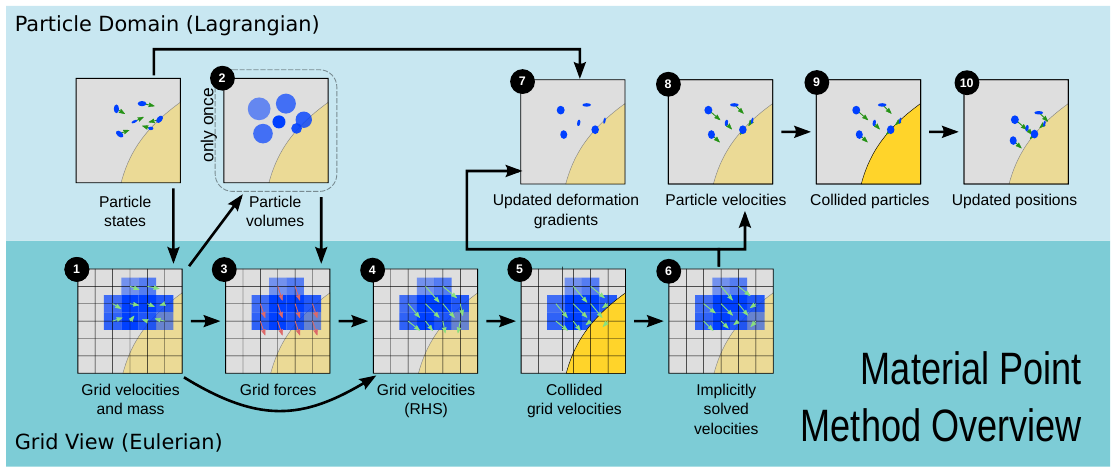
\includegraphics[height=5cm]{MPMOverview.png}\\

~\\

\begin{itemize}

\item Continuum based particle method with background mesh for gradients\\

\item Extension of FLIP (which is an extension of PIC)\\

\item Used in rendering for the movie \emph{Frozen}\\

\end{itemize}

\end{center}
\end{frame}

%------------------------------------------------

\begin{frame}
\begin{center}
\frametitle{What does MPM have to do with FEM?}

\begin{itemize}

\item Problem on background mesh changes when material points move\\

~\\

\item Natural fit for matrix-free representation\\

~\\

\item Similar reasoning to use matrix-free for adaptive methods\\

~\\

\item Ratel/libCEED FEM infrastructure provides fast background mesh solves\\

\end{itemize}

\end{center}
\end{frame}

%------------------------------------------------

\begin{frame}
\begin{center}
\frametitle{libCEED Basis Evaluation AtPoints}

\begin{center}
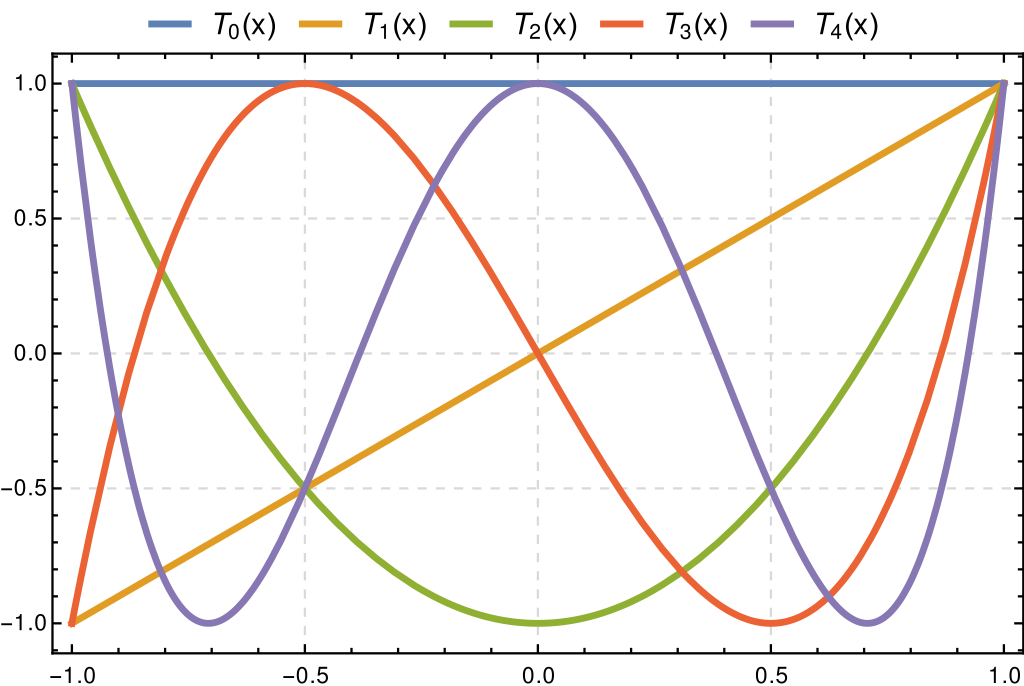
\includegraphics[height=4cm]{ChebyshevPolynomials.png}
\end{center}

\begin{itemize}

\item Interpolate from primal to dual (quadrature) space\\

\item Fit Chebyshev polynomials to values at quadrature points\\

\item Evaluate Chebyshev polynomials at reference coords of material points\\

\item Transpose the order for projection to mesh from material points\\

\end{itemize}

\end{center}
\end{frame}

%------------------------------------------------
\subsection{Shared Memory Bases}
%------------------------------------------------

\begin{frame}[fragile]
\begin{center}
\frametitle{Shared Basis Code}

{\tiny
\begin{lstlisting}[style=boxedC]
extern "C" __launch_bounds__(BASIS_INTERP_BLOCK_SIZE) __global__
    void InterpAtPoints(const CeedInt num_elem, const CeedScalar *c_B,
    const CeedInt *points_per_elem, const CeedScalar *__restrict__ d_X,
    const CeedScalar *__restrict__ d_U, CeedScalar *__restrict__ d_V) {
  // Setup (omitted)
  // Apply basis element by element
  for (CeedInt elem=blockIdx.x*blockDim.z+threadIdx.z; elem<num_elem; elem+=gridDim.x*blockDim.z) {
    // Map from nodes to Chebyshev coefficients
    ReadElementStrided2d<NUM_COMP,P_1D>(data,elem,1,P_1D*P_1D*num_elem,P_1D*P_1D,d_U,r_U);
    InterpTensor2d<NUM_COMP,P_1D,Q_1D>(data,r_U,s_B,r_C);
    // Map from Chebyshev coefficients to points
    for (CeedInt i=threadIdx.x+threadIdx.y*blockDim.x; i<point_loop_bound; i+=blockDim.x*blockDim.y) {
      const CeedInt p = i % NUM_PTS;
      ReadPoint<DIM,NUM_PTS>(data,elem,p,NUM_PTS,1,num_elem*NUM_PTS,NUM_PTS,d_X,r_X);
      InterpAtPoints2d<NUM_COMP,NUM_PTS,Q_1D>(data,i,r_C,r_X,r_V);
      WritePoint<NUM_COMP,NUM_PTS>(data,elem,p,NUM_PTS,1,num_elem*NUM_PTS,NUM_PTS,r_V,d_V);
    }
  }
}
\end{lstlisting}
}

Threadblock maps to Chebeshev coeffs on element (standard interpolation)\\

~\\

Each thread maps from Chebyshev coeffs to single point\\

\end{center}
\end{frame}

%------------------------------------------------

\begin{frame}[fragile]
\begin{center}
\frametitle{Shared Basis Code}

{\tiny
\begin{lstlisting}[style=boxedC]
template <int NUM_COMP, int NUM_POINTS, int Q_1D>
inline __device__ void InterpAtPoints2d(SharedData_Hip &data, const CeedInt p, const CeedScalar *__restrict__ r_C, const CeedScalar *__restrict__ r_X,
                                        CeedScalar *__restrict__ r_V) {
  for (CeedInt i = 0; i < NUM_COMP; i++) r_V[i] = 0.0;
  for (CeedInt comp = 0; comp < NUM_COMP; comp++) {
    CeedScalar buffer[Q_1D];
    CeedScalar chebyshev_x[Q_1D];
    // Load coefficients
    if (data.t_id_x<Q_1D && data.t_id_y<Q_1D) {
      data.slice[data.t_id_x+data.t_id_y*Q_1D] = r_C[comp];
    }
    __syncthreads();
    // Contract x direction
    ChebyshevPolynomialsAtPoint<Q_1D>(r_X[0], chebyshev_x);
    for (CeedInt i = 0; i < Q_1D; i++) {
      buffer[i] = 0.0;
      for (CeedInt j = 0; j < Q_1D; j++) {
        buffer[i] += chebyshev_x[j] * data.slice[j + i*Q_1D];
      }
    }
    // Contract y direction
    ChebyshevPolynomialsAtPoint<Q_1D>(r_X[1], chebyshev_x);
    for (CeedInt i = 0; i < Q_1D; i++) {
      r_V[comp] += chebyshev_x[i] * buffer[i];
    }
  }
}
\end{lstlisting}
}

Each thread (point) needs separate contraction buffers\\

\end{center}
\end{frame}

%------------------------------------------------
\section{Operator Assembly}
%------------------------------------------------

\begin{frame}
\begin{center}
\frametitle{Preconditioning Support}

Some operator assembly needed for preconditioning\\

~\\

Diagonal assembly for Jacobi, Chebyshev\\

~\\

Full assembly for AMG or LU\\

\end{center}
\end{frame}

%------------------------------------------------
\subsection{Diagonal Assembly}
%------------------------------------------------

\begin{frame}
\begin{center}
\frametitle{FEM Diagonal Assembly}

FEM diagonal assembly consists of two phases\\

~\\

\begin{itemize}

\item QFunction assembly\\

\begin{itemize}

\item Assemble small matrix at each quadrature point\\

\item Each active input individually set to 1\\

\item QFunction kernel ${\color{applegreen}D}$ called to populate assembled row\\

\end{itemize}

~\\

\item Diagonal assembly\\

\begin{itemize}

\item Compute diagonal entries of ${\color{blue(ncs)}B}^T {\color{applegreen}D} {\color{blue(ncs)}B}$ on element\\

\item Element diagonals assembled via $\mathcal{E}^T$ for local diagonal\\

\end{itemize}

\end{itemize}

\end{center}
\end{frame}

%------------------------------------------------

\begin{frame}
\begin{center}
\frametitle{MPM Diagonal Assembly}

MPM diagonal assembly consists of a single phase\\

~\\

\begin{itemize}

\item Each input node on elements individually set to 1\\

~\\

\item Basis ${\color{blue(ncs)}B}$ applied to get values at material points\\

~\\

\item QFunction kernel ${\color{applegreen}D}$ called to populate result\\

~\\

\item Basis ${\color{blue(ncs)}B}^T$ applied to get values at nodes\\

~\\

\item Corresponding diagonal entry copied into element diagonal\\

~\\

\item Element diagonals assembled via $\mathcal{E}^T$ for local diagonal\\

\end{itemize}

\end{center}
\end{frame}

%------------------------------------------------
\subsection{Full Assembly}
%------------------------------------------------

\begin{frame}
\begin{center}
\frametitle{FEM Full Assembly}

FEM full assembly consists of three phases\\

~\\

\begin{itemize}

\item Sparsity pattern\\

\begin{itemize}

\item Compute local (on process) matrix COO indices for entries\\

\end{itemize}

~\\

\item QFunction assembly\\

\begin{itemize}

\item Same as for diagonal assembly\\

\end{itemize}

~\\

\item Full assembly\\

\begin{itemize}

\item Compute entries of ${\color{blue(ncs)}B}^T {\color{applegreen}D} {\color{blue(ncs)}B}$ for each element\\

\item Populate assembled array per the sparsity pattern\\

\end{itemize}

\end{itemize}

\end{center}
\end{frame}

%------------------------------------------------
\section{Questions}
%------------------------------------------------

\begin{frame}
\frametitle{Questions?}

\begin{center}
\includegraphics[height=2.75cm]{libCEEDlogo.png}
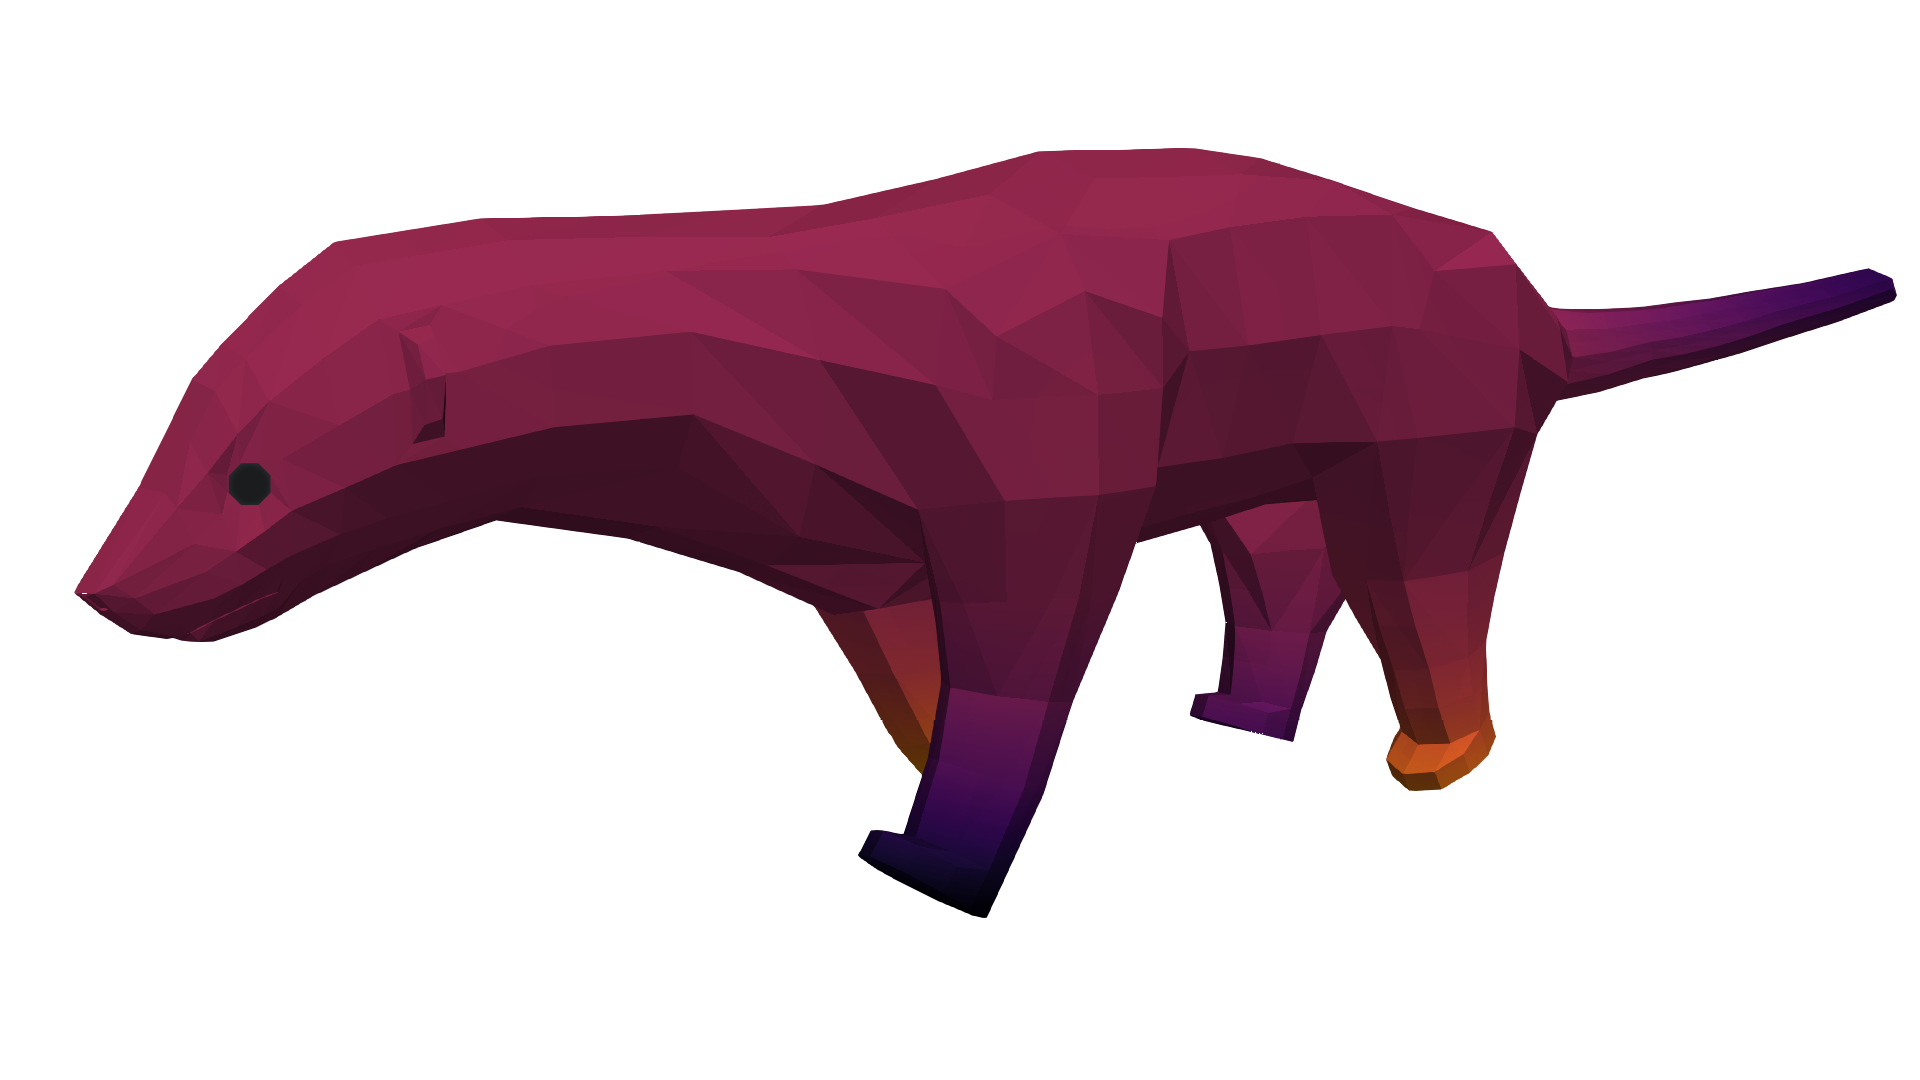
\includegraphics[height=2.75cm]{Ratellogo.png}
\end{center}

{\flushleft

libCEED Repo: https://github.com/CEED/libCEED\\
HONEE Repr: https://gitlab.com/phypid/HONEE\\
Ratel Repo: https://gitlab.com/micromorph/ratel\\

~\\

Grant: Predictive Science Academic Alliance Program (DE-NA0003962)\\

}

\begin{center}

\includegraphics[height=0.8cm]{psaap-center-logos}
\end{center}

\end{frame}

%-------------------------------------------------------------------------------

\end{document}

%-------------------------------------------------------------------------------
